\begin{figure}[ht]
  \centerline{
    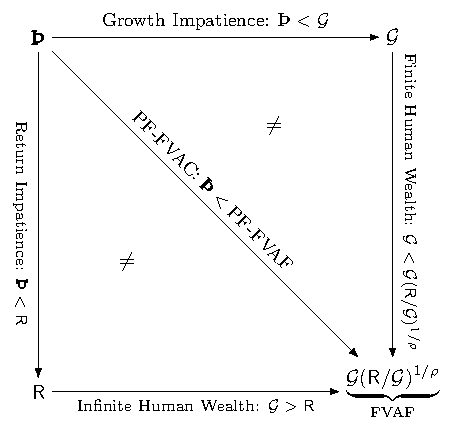
\includegraphics[width=5in]{Figures/RelatePFGICFHWCRICPFFVAC}
  }
  \caption{Perfect Foresight Relation of Consumer Patience Conditions}
  \label{fig:RelatePFGICFHWCRICPFFVAC}
%  \iflabelexists{fig:RelatePFGICFHWCRICPFFVAC}{}{\label{fig:RelatePFGICFHWCRICPFFVAC}}
    % Don't define it if already defined
  \footnotesize{The acronyms in this figure refer to each of the consumer patience conditions in the perfect foresight case. Refer to Table~\ref{table:Comparison} for their definitions. An arrowhead points to the larger of the two quantities being compared; so, following the diagonal arrow imposes that absolute patience is smaller than the limit defined by the finite value of autarky factor, $\APFac < \PermGroFac (\Rfree/\PermGroFac)^{1/\CRRA}$ (this is one way of writing the {\PFFVAC}, equation \eqref{eq:PFFVAC}}). (The $\neq$ symbols indicate that the diagram is not commutative; that is, the different ways of reaching the conclusion that the {\PFFVAC} holds are not equivalent to each other).
\end{figure}
